\documentclass[compress,unicode]{beamer}
\usepackage[utf8]{inputenc}
\usepackage[russian]{babel}
\usepackage{cmap}
\usepackage{nicefrac}
\usepackage{tikz}
\usepackage{pscyr}
\usepackage{listings}
\usetikzlibrary{shapes,snakes,trees,positioning}




\definecolor{linenum}{rgb}{0.4,0.4,0.6}
\definecolor{keywords}{rgb}{0.2,0.2,0.4}
\definecolor{firstlevel}{rgb}{0.4,0,0}
\definecolor{secondlevel}{rgb}{0.7,0,0}
\definecolor{thirdlevel}{rgb}{1,0,0}
\definecolor{main}{rgb}{0.3,0.45,0.6}

\lstdefinestyle{mystyle}{language=Python,
numbers=left,
numberstyle=\tiny\color{linenum},
numbersep=5.5pt,
keywordstyle=\bf\color{keywords}}
\lstdefinelanguage{morepython}
{morekeywords={map,sorted}}

\usetheme{Warsaw}
\usecolortheme[RGB={150,150,200}]{structure} 
\setbeamercolor*{palette primary}{use=structure,fg=white,bg=main}
 \setbeamertemplate{blocks}[rounded][shadow=true] 
%\setbeamercolor{frametitle}{fg=white,bg=main}
%\setbeamercolor{outline}{fg=white,bg=main}
%\setbeamercolor{title}{fg=white,bg=main}

\usepackage{verbatim}
\usepackage[margin=15pt,font={small,sf,it},labelfont=bf]{caption} 
\usebackgroundtemplate{
\includegraphics[width=\paperwidth]{drawing.png}}

\setbeamersize{text margin left=1.5em,text margin right=1.5em}
\setbeamertemplate{itemize item}{$\bullet$}
\setbeamertemplate{itemize subitem}{$\bullet$}
\setbeamertemplate{enumerate items}[default]

\setbeamercolor{enumerate item}{bf=black,fg=main}  
\setbeamercolor{itemize item}{fg=main}  
\setbeamercolor{enumerate subitem}{bf=white,fg=main}  
\setbeamercolor{itemize subitem}{fg=main} 

\useoutertheme[subsection=false]{smoothbars}
\title[Машинное обучение]{Кластеризация. Графовый подход, EM и k means, иерархическая кластеризация}
\author{Сергей Лисицын}
\institute{lisitsyn.s.o@gmail.com}
\date{\today}
\setbeamertemplate{footline}[page number]{}
\setbeamertemplate{navigation symbols}{}
%\renewcommand{\sfdefault}{fma}
\begin{document}
\section{}
\abovedisplayskip=.6\abovedisplayskip
\belowdisplayskip=.6\belowdisplayskip

\begin{frame}

\titlepage
\end{frame}

\section{Общие понятия}
\subsection{}
\begin{frame}{Задача кластеризации}{Clustering}
\begin{itemize}
	\item Имеется некоторое множество объектов 
	\item Решением задачи является некоторое разбиение множества на непересекающиеся кластеры
	\item Кластеры -- некоторые характерные группы объектов
	\item Количество кластеров для разбиения может быть задано изначально
	\item Эффективность разбиения оценивается функционалами внутриклассового и межклассового расстояния
	\item Задача ещё более некорректна чем классификация
\end{itemize}
\end{frame}

\begin{frame}{Общая задача кластеризации}

Пусть имеется некоторое множество объектов $\mathcal{X}$ и конечное множество кластеров $\mathcal{C}$. 
Необходимо найти функциональную зависимость
$$
f: \mathcal{X} \to \mathcal{C},
$$
причём (в отличие от классификации) ни одно значение $f$ на $\mathcal{X}$ априори не известно. \\[10pt]

В {\color{main!20!black}\bf задаче кластеризации} функция $f$ должна быть построена таким образом, чтобы выделять наиболее характерные группы объектов. 

\end{frame}

\begin{frame}{Свойства кластеров}
\begin{tabular}{p{8cm}c}
Компактность (compactness): \small кластеры компактны -- объекты лежат внутри некоторого плотного множества & \parbox{3cm}{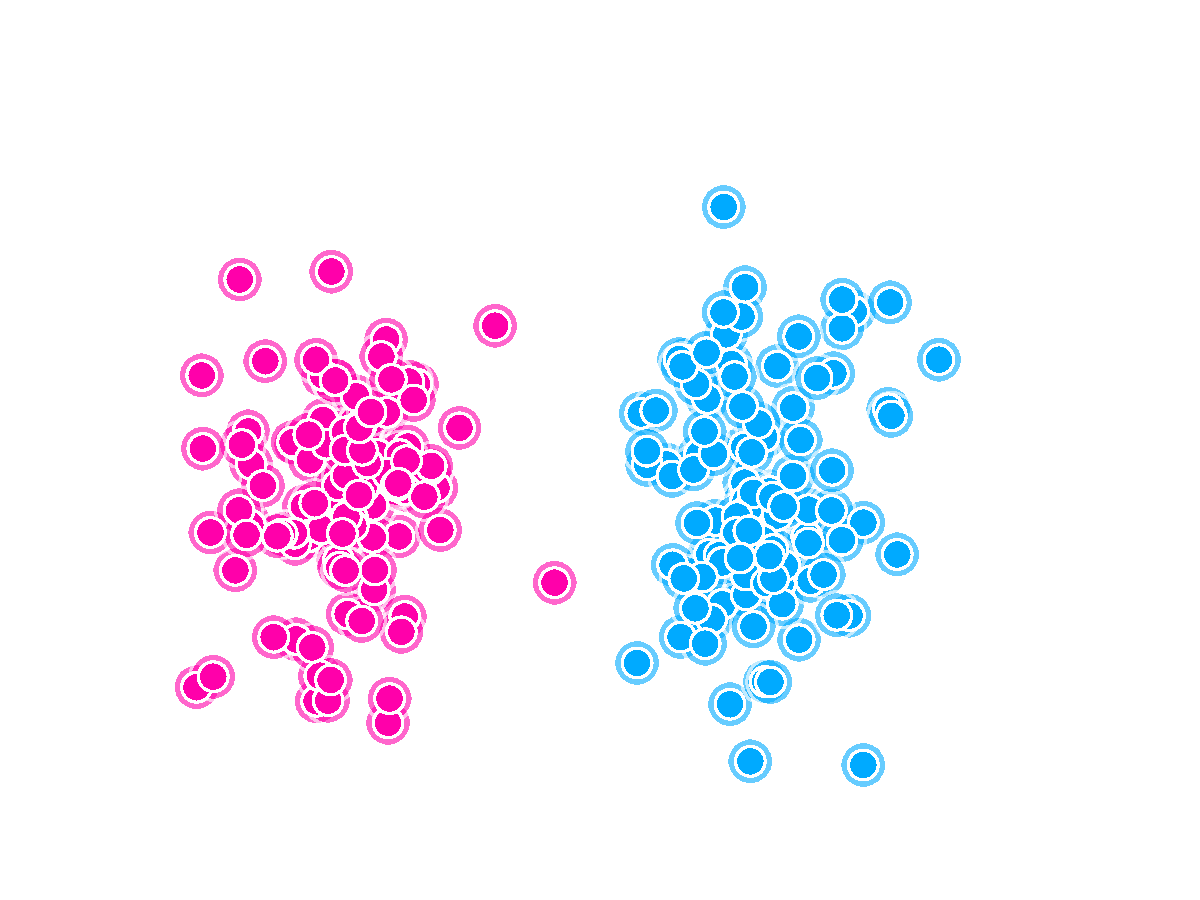
\includegraphics[width=3cm]{compactness}}\\
Связность (connectivity): \small объекты кластера можно выделить в связные структуры & \parbox{3cm}{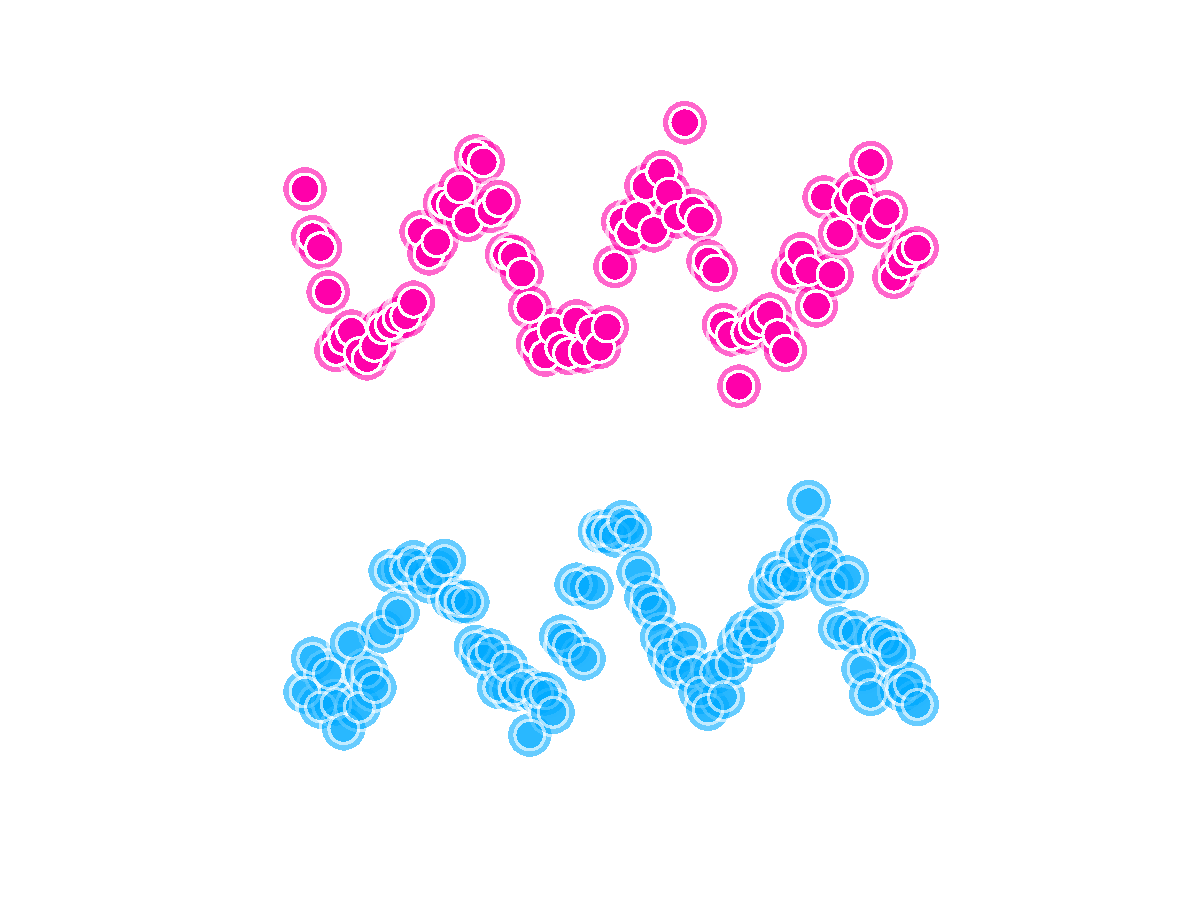
\includegraphics[width=3cm]{connectivity}} \\
Пространственное разделение (spatial separation): \small кластеры отстоят друг от друга на некотором расстоянии & \parbox{3cm}{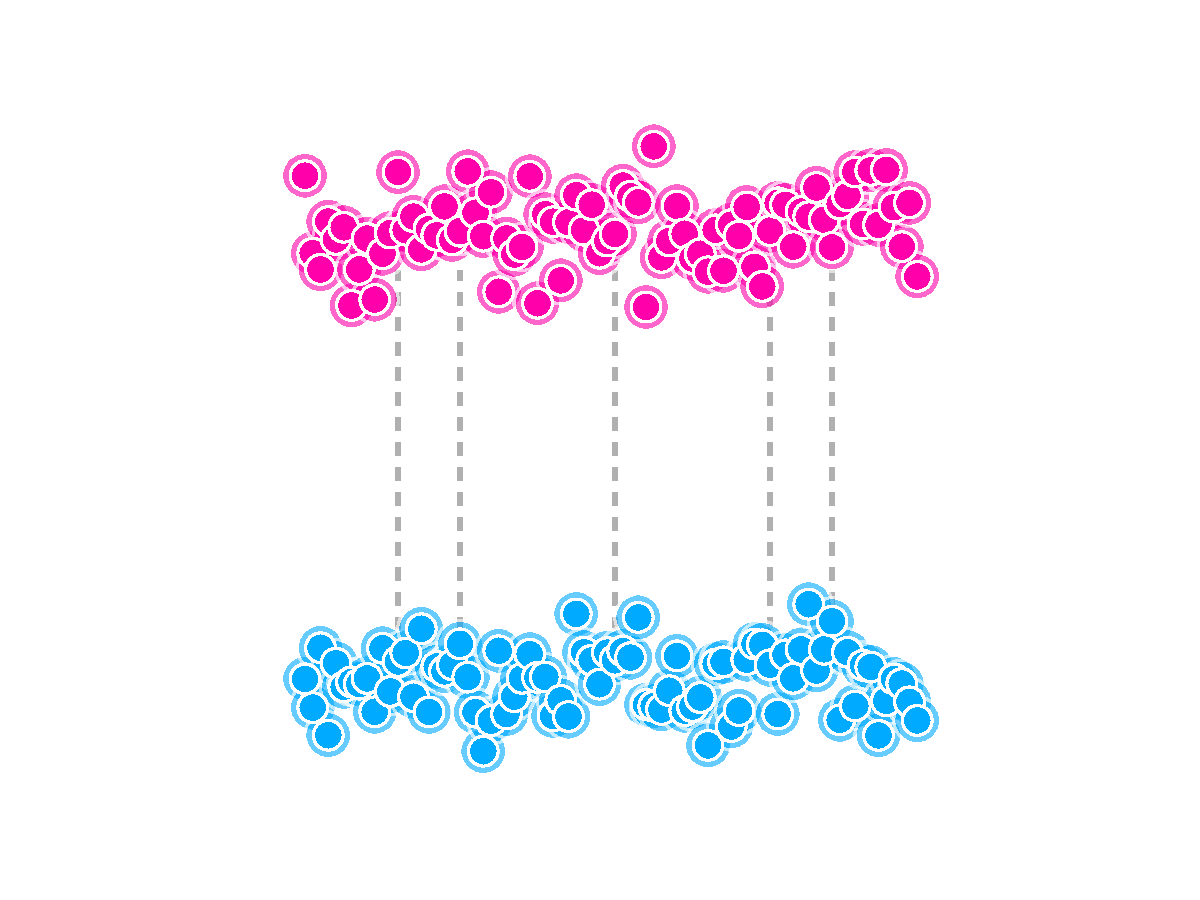
\includegraphics[width=3cm]{spatial-sep}}
\end{tabular}

\end{frame}

\begin{frame}{Функционалы качества кластеризации}
\begin{itemize}
	\item{Межкластерное расстояние}
	$$
	\rho_c(c_1,c_2) = \sum_{f(x_1) = c_1 , f(x_2) = c_2} \rho(x_1,x_2)
	$$
	Эффективная кластеризация подразумевает максимизацию межкластерных расстояний:
	$
	\sum_{\substack{c_1 \ne c_2 \\ c_1,c_2 \in \mathcal{C}}} \rho_c(c_1,c_2) \to \max
	$
	\item{Внутрикластерное расстояние}
	$$
	\rho_{\mathsf{inner}} (c) = \sum_{f(x_1)=f(x_2) = c} \rho(x_1,x_2)
	$$
	Эффективная кластеризация подразумевает минимизацию внутрикластерных расстояний: 
	$
	\sum_{c\in \mathcal{C}} \rho_{\mathsf{inner}} (c) \to \min 
	$
	\item В некоторых случаях минимизируется отношение межкластерного и внутрикластерного расстояний

\end{itemize}
\end{frame}



\begin{frame}{Цели кластеризации}
\begin{itemize}
	\item Выделение наиболее характерных групп объектов
	\item Выяснение структуры множества объектов
	\item Сокращение объема выборки объектов
	\item Обнаружение <<необычных>> объектов (novelty detection)

\end{itemize}

\end{frame}



\section{Графофые алгоритмы}
\subsection{}
\begin{frame}{Графовый подход к кластеризации}
\begin{itemize}
	\item Множество объектов в метрическом пространстве представимо в виде неориентированного взвешенного графа, где вес ребра это значение метрики между его объектами-вершинами
	\item Кластеры в таком графе -- непересекающиеся подграфы исходного
	\item Графы сами по себе достаточно удобны для кластеризации
	\item Представление объектов в таком случае знать не обязательно, достаточно расстояний между ними, вычисленных даже косвенно
	\item Кроме того, такие графы-кластеры удобно визуализировать
%\begin{tikzpicture}
\tikzstyle{point}=[circle,fill=black!25,minimum size=17pt,inner sep=0pt]
\tikzstyle{1-point}=[point,fill=main]

\foreach \x / \y in 
{
-2.7/2.1,
-3.1/3.2,
-2.1/1.6,
-1.9/3.1
}
\node[1-point,minimum size = 15pt, fill = main!80!black] () at (\x,\y) {}
node[1-point,minimum size=12pt, fill=main!20] () at (\x,\y) {};

\foreach \x / \y in 
{
0.3/2.1,
-0.1/3.2,
0.9/1.6,
1.1/3.1
}
\node[1-point,minimum size = 15pt, fill = main!80!black] () at (\x,\y) {}
node[1-point,minimum size=12pt, fill=main!20] () at (\x,\y) {};

\end{tikzpicture}

\end{itemize}
\end{frame}

\subsection{}
\begin{frame}{Алгоритм выделения связных компонент}
\begin{itemize}
\item Кластеры в пространстве можно представлять как группы связных объектов некоторого графа -- связные компоненты
\item Связная компонента -- подграф, в котором все вершины взаимно достижимы
\item Удаляя (или не создавая) ребра графа с весом, большим, чем некоторый параметр $R_{max}$, можно разбить граф на некоторое количество связных компонент
\item В распавшемся графе будут выделены некоторые характерные структуры с минимальным внутрикластерным расстоянием
\end{itemize}
\end{frame}

\begin{frame}{Описание алгоритма выделения связных компонент}{}
\begin{block}{}
\small
{\bf\color{main}Вход:} множество объектов $\mathcal{X}$, параметр $R_{max}$ \\
{\bf\color{main}Выход:} множество пар (объект-кластер) \\
\begin{enumerate}
\item Создать граф без ребёр с узлами, соответствующими элементам множества $\mathcal{X}$
\item Соединить все узлы графа, соответствующие элементам $x_i, x_j \in \mathcal{X}, \forall_{i \ne j}$, для которых $\rho(x_i,x_j) < R_{max}$
\item Возвратить соответствующие вершинам графа пары (элемент множества $\mathcal{X}$ -- номер связной компоненты)
\end{enumerate}
\end{block}
\end{frame}

\begin{frame}{}
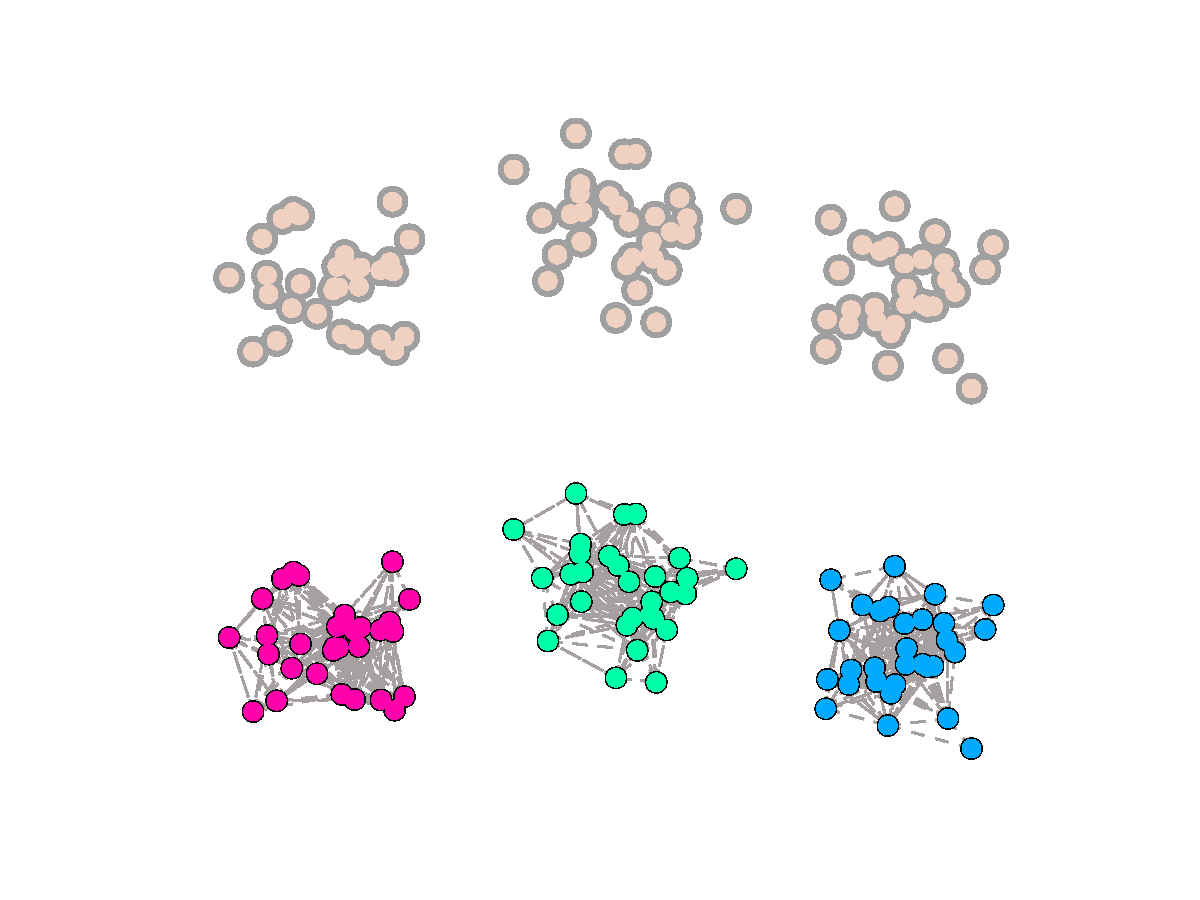
\includegraphics[width=\textwidth]{connected-components-clustering}
\end{frame}

\begin{frame}{}
\begin{block}{}
\scriptsize
\lstinputlisting[style=mystyle,fontadjust,alsolanguage=morepython]{CCclusterer.py}
\end{block}
\end{frame}


\subsection{}
\begin{frame}{Алгоритм построения покрывающего дерева}{Spanning tree clustering}
\begin{itemize}
	\item Минимальное покрывающее дерево -- древовидная структура с минимальным суммарным расстоянием между соседними объектами
	\item При удалении из построенного дерева $K-1$ самых <<длинных>> ребёр максимизируется межкластерное расстояние
	\item Минимум суммарного расстояния между объектами минимизирует внутрикластерное расстояние
	\item Количество кластеров в таком случае задаётся заранее, алгоритм ведёт себя предсказуемее
\end{itemize}
\end{frame}

\begin{frame}{Описание алгоритма кластеризации с помощью минимального покрывающего дерева}{}
\begin{block}{}
\small
{\bf\color{main}Вход:} множество объектов $\mathcal{X}$, параметр $K$ -- количество кластеров\\
{\bf\color{main}Выход:} множество пар (объект-кластер) \\
\begin{enumerate}
\item Построить минимальное покрывающее дерево c узлами $0,1,\dots$, для которого 
$$
\sum_{i,j} \rho (x_i,x_j) \to \min 
$$
\item Удалить $K-1$ ребёр $(i,j)$ максимальной метрики $\rho(x_i,x_j)$ построенного покрывающего дерева
\item Возвратить соответствующие вершинам графа пары (элемент множества $\mathcal{X}$ -- номер связной компоненты)

\end{enumerate}
\end{block}\end{frame}


\begin{frame}{}
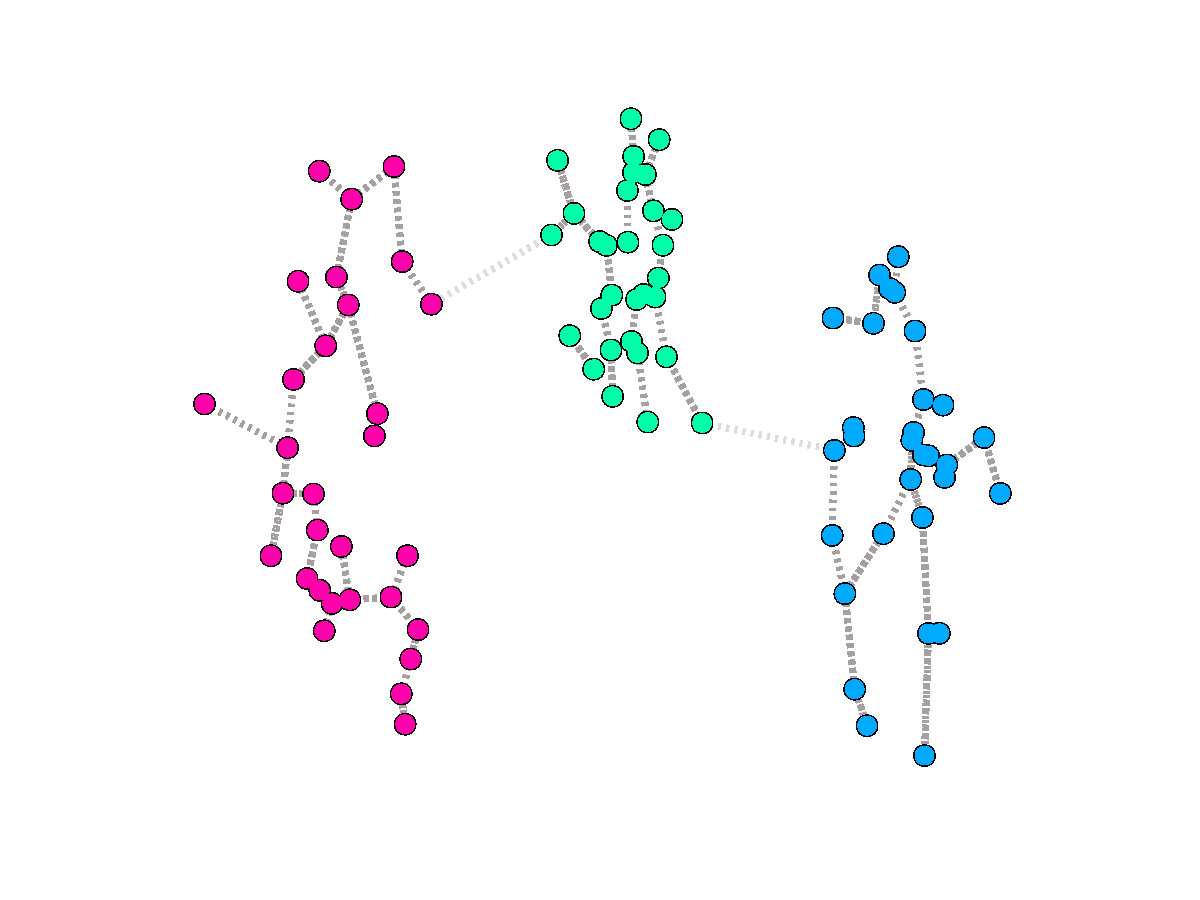
\includegraphics[width=\textwidth]{spanning-tree-clustering}
\end{frame}

\begin{frame}{}
\begin{block}{}
\scriptsize
\lstinputlisting[style=mystyle,fontadjust,alsolanguage=morepython]{STclusterer.py}
\end{block}
\end{frame}



\begin{frame}{Пример социальной кластеризации}
\begin{itemize}
	\item Объекты пространства -- пользователи социальной сети (электронной почты, ICQ, etc)
	\item Никакой информации о самих объектах не имеется, можно определить только расстояния между объектами
	\item Метрика между двумя пользователями может определяться как обратное нормированное количество сообщений между ними
	\item Результатом кластеризации будут группы людей, наиболее тесносвязанные друг с другом (можно на это надеяться)
\end{itemize}
\end{frame}

\begin{frame}{Пример социальной кластеризации}
\begin{tikzpicture}[overlay]
\node at (5.92,-0.68) { 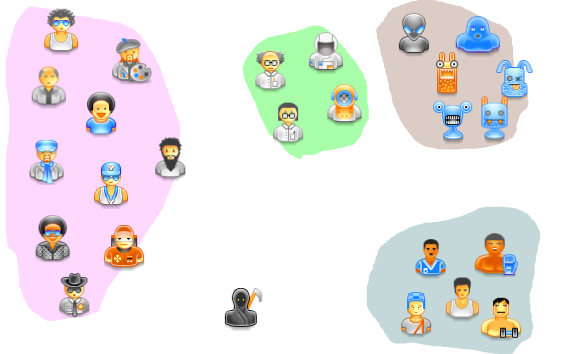
\includegraphics[width=1.18\textwidth]{people}} ;
\end{tikzpicture}
\end{frame}

\begin{frame}{Эффективность алгоритмов}
\begin{itemize}
	\item Для обоих алгоритмов необходимо найти все взаимные метрики за $O(n^2)$, выделение кластеров выполняется поиском в ширину или глубину $O(|V|+|E|)$ (однако для построения покрывающего дерева существуют особые алгоритмы)
	\item Оба алгоритма неустойчивы к близкорасположенным кластерам -- нет <<баланса>> между уменьшением функционалов качества, минимизируется только внутрикластерное расстояние
	\item Алгоритм выделения связных компонент плохо обусловлен по своему параметру $R_{max}$: небольшие изменения $R_{max}$ могут повлечь резкое увеличение или уменьшение количества кластеров
	\item Алгоритм кластеризации с помощью покрывающего дерева выделяет заданное количество кластеров
\end{itemize}
\end{frame}


%\begin{frame}{Алгоритм ФОРЭЛ}{}
%\pgfdeclaremask{mymask}{alaska-rainbow-trout-mask}
%\pgfimage[mask=mymask,width=\textwidth]{alaska-rainbow-trout.jpg}
%\end{frame}


%\begin{frame}{Алгоритм ФОРЭЛ}{{\bf фор}мальный {\bfэл}емент}
%\begin{itemize}
%\item Метод был предложен в 1967 советскими математиками Н.Г. Загоруйко и В.Н. %Ёлкиной
%\item Предполагает использование некоторых условно существующих, формальных %элементов пространства объектов
%\item Пространство объектов должно быть не только метрическим, но и линейным: %требуется операция сложения объектов и умножения на вещественное число
%\item Не основан на графах, использует графовый метод кластеризации на %последнем этапе работы
%\end{itemize}
%\end{frame}

%\begin{frame}{Описание алгоритма}
%\begin{block}{}
%\small
%{\bf\color{main}Вход:} множество объектов $\mathcal{X}$, параметр $R$ -- радиус кластера, количество кластеров $K$\\
%{\bf\color{main}Выход:} множество пар (кластер, множество объектов кластера) %\\
%\begin{enumerate}
%\item Пока остались остались некластеризованные объекты
%\begin{itemize}
%	\item Определить в пространстве объектов элемент $x_0$
%	\item Выделить все $x$, для которых $\rho (x_0, x) < R$ в множество %$\mathcal{C}_0$ и переместить точку в центр $\mathcal{C}_0$: $\displaystyle %x_0 = \frac{1}{|\mathcal{C}_0|} \sum_{x\in\mathcal{C}_0} x$
%	\item Исключить все объекты множества $\mathcal{C}_0$ из кластеризуемых %объектов, а сам объект $x_0$ запомнить
%\end{itemize}
%\item Из формальных элементов $x_0^{(i)}$ составить граф, по которому провести %кластеризацию (например покрывающим деревом) с параметром количества кластеров %$K$
%\item Все объекты отнести к классу ближайшего к нему формального элемента %$x_0^{(i)}$
%\end{enumerate}
%\end{block}
%\end{frame}





\section{EM $\rightarrow$ k-means}
\subsection{}

\begin{frame}{Смеси распределений}
\begin{itemize}
\item Выборка с группами может рассматриваться как группа нескольких многомерных распределений, такое предположение задаёт общую плотность распределения
$$
p(x) = \sum_c P(c) p_c (x),
$$
где $p_c (x)$ -- функция плотности распределения кластера $c$, а $P(c)$ -- априорная вероятность класса
\item Кластер объектов --  компонента этой смеси распределений с плотностью $f_c$
\item Кластеризация сводится к нахождению компонент смеси распределений по эмпирическим оценкам плотности, а принадлежность конкретных объектов определяется максимумом $P(c) p_c(x)$
\end{itemize}

\end{frame}



\begin{frame}{EM-алгоритм}{Expectation-Maximization}
\begin{itemize}
	\item Описан в 1977 году Демпстером, Лэйрдом и Рабином и предназначен для оценок максимального правдоподобия в статистических моделях
	\item В случае кластеризации EM-алгоритм позволяет найти компоненты смеси распределений
	\item По полученным компонентам смеси распределений классификация производятся достаточно легко
	\item Для кластеризации, как правило используют гауссианы:
	$$p_c (x) = \mathcal{N} (x, \mu_c, \mathbf{R}_c)$$
	\item Алгоритм итеративен и выполняется до тех пор, пока всем объектам не будут назначены <<стабильные>> кластеры, не изменяющиеся в течение следующих итераций

\end{itemize}
\end{frame}

\begin{frame}{}
\begin{block}{}
\footnotesize
{\bf\color{main}Вход:} множество объектов $\mathcal{X}$, количество кластеров $k$\\
{\bf\color{main}Выход:} множество пар (объект-кластер) \\
\begin{enumerate}
\item Задать начальные приближения $P(c) = 1/k$, за $\mu_c$ принять случайные объекты выборки, рассчитать $diag~\mathbf{R_c} = \frac{\sum_{x \in \mathcal{X}} g_c (x)  (x- \mu_c)^2}{|\mathcal{X}| P(c)} $
\item До тех пор, пока кластеры не стабилизируются:
\begin{enumerate}
\footnotesize
\item E-шаг\\
{
\color{main!30!black}Вычисление апостериорных вероятностей
$$
g_c = \frac{P(c) \mathcal{N} (x,\mu_c, \mathbf{R}_c)}{\sum_k P(k) \mathcal{N}(x,\mu_k,\mathbf{R}_k)}
$$
}
\item M-шаг\\
{\footnotesize
\color{main!30!black}Пересчёт параметров гауссианов

\begin{multline*}
P(c) = \frac{\sum_x g_c (x)}{|\mathcal{X}|} , ~~~
 \mu_c = \frac{\sum_x g_c (x) x}{|\mathcal{X}| P(c)}    ,~~~ diag~\mathbf{R_c} = \frac{\sum_{x \in \mathcal{X}} g_c (x)  (x- \mu_c)^2}{|\mathcal{X}| P(c)} 
\end{multline*}
}
\item Для каждого объекта выбрать кластер $\arg \max_c g_c$
\end{enumerate}
\end{enumerate}
\end{block}
\end{frame}

\begin{frame}{Эффективность}
\begin{itemize}
	\item Алгоритм EM в самом общем виде не очень практичен
	\item В случае плохого выбора скрытых переменных и неправильной оценки количества кластеров алгоритм плохо сходится
	\item Алгоритм очень трудоёмок в вычислениях
	\item Итеративная природа алгоритма требует определять либо количество итераций, либо критерий останова
\end{itemize}
\end{frame}

\begin{frame}{Алгоритм кластеризации k средних}{k means clustering}
\begin{itemize}
	\item Является упрощенным вариантом EM-алгоритма
	\item Идея алгоритма состоит в <<стабилизации>> центров кластеров на M-шаге и жёсткой привязке объектов к ближайшему центру на E-шаге
%	\item Сходимость суперполиномиальная
	\item Алгоритм итеративен: выбирается либо количество итераций, либо условие сходимости
	\item Выделяет только заданное количество компонент, но существуют модификации для переменного параметра $k$
\end{itemize}
\end{frame}

\begin{frame}{}
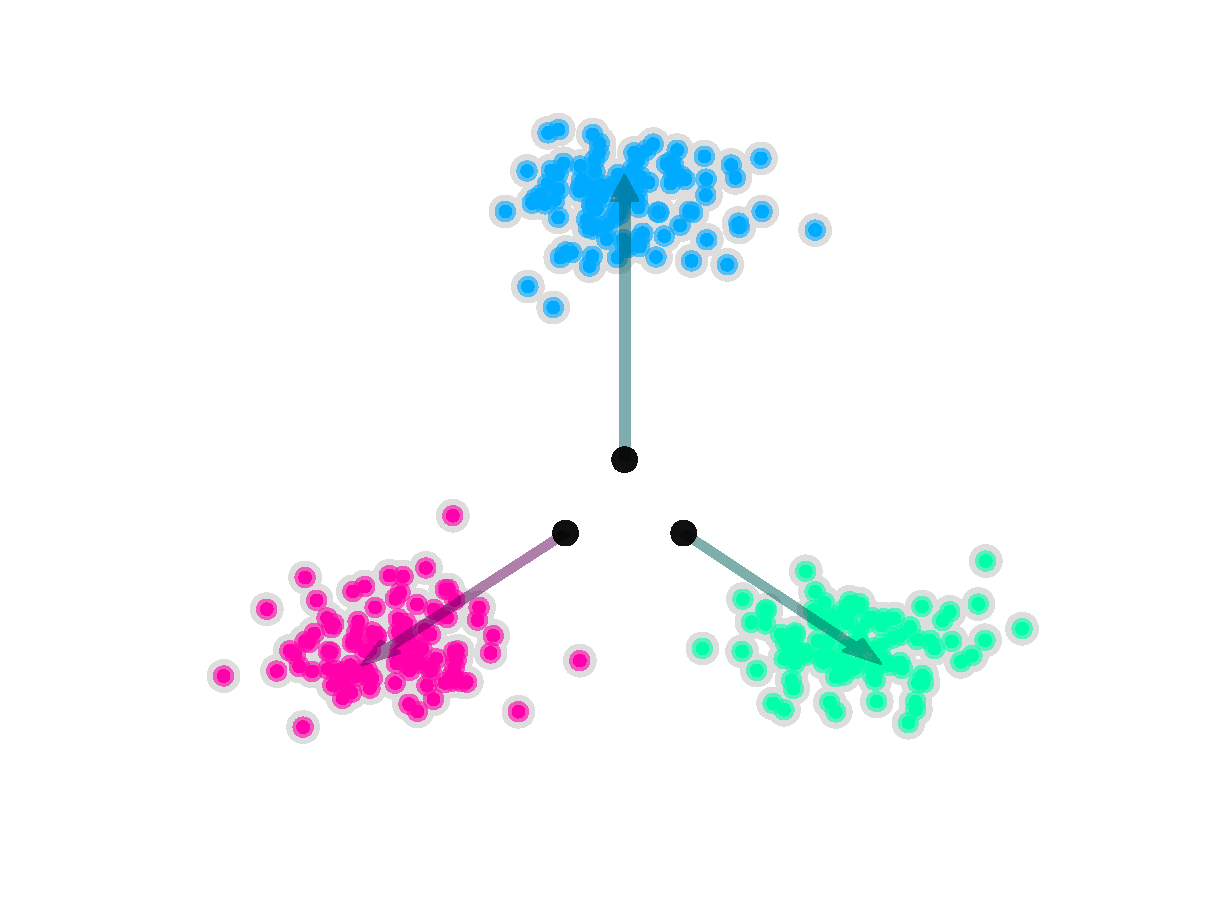
\includegraphics[width=\textwidth]{k-means}
\end{frame}

\begin{frame}{Описание алгоритма k средних}
\begin{block}{}
\small
{\bf\color{main}Вход:} множество объектов $\mathcal{X}$, количество центроидов $k$, количество итераций или условие останова алгоритма \\
{\bf\color{main}Выход:} множество пар (объект-кластер) \\
\begin{enumerate}
\item Занести в множество центроидов $\mathbf{C}$ случайные объекты из $\mathcal{X}$, не изменяя $\mathcal{X}$
\item До тех пор, пока центроиды не стабилизировались (или не выполнилось заданное количество итераций):
\begin{enumerate}
	\item Для каждого объекта $x\in \mathcal{X}$: задать объекту $x$ ближайший к нему центроид $c$: $f(x) = c, ~ \rho(c,x) \to \min_c$
	\item Для каждого центроида $c \in \mathbf{C}$: пересчитать положение 
	$$
	c = \frac{\sum_{x, f(x)=c} x}{\sum_{x, f(x)=c} 1}
	$$
	

\end{enumerate}
\item Вернуть пары (объект из $\mathcal{X}$ -- номер ближайшего к нему центроида)
\end{enumerate}
\end{block}
\end{frame}

\begin{frame}{}
\begin{block}{}
\scriptsize
\lstinputlisting[style=mystyle,fontadjust,alsolanguage=morepython]{KMeansclusterer.py}
\end{block}
\end{frame}
\begin{frame}{Кластеризация целей}
\begin{itemize}
\item Имеется $k$ боеприпасов некоторого вооружения, нанесём удары в наиболее сосредоточенные группы объектов
\item Необходимо выделить объекты на изображении -- но это задача соседней области -- computer vision
\item В случае неверной кластеризации боеприпас будет потрачен зря: либо нанесёт удар в пустое пространство, либо нанесёт лишний удар по одной точке
\item Однако, лучше, когда $k$ больше, чем групп объектов

\end{itemize}
\end{frame}

\begin{frame}{Кластеризация целей: изначальный снимок}
\begin{tikzpicture}[overlay]
\node at (5.85,-0.56) { \includegraphics[width=1.18\textwidth]{raw}} ;
\end{tikzpicture}
\end{frame}

\begin{frame}{Кластеризация целей: выделение объектов}
\begin{tikzpicture}[overlay]
\node at (5.85,-0.56) { \includegraphics[width=1.18\textwidth]{raw_2}} ;
\end{tikzpicture}
\end{frame}

\begin{frame}{Кластеризация целей: k=8}
\begin{tikzpicture}[overlay]
\node at (5.85,-0.575) { \includegraphics[width=1.18\textwidth]{k-means-2}} ;
\end{tikzpicture}
\end{frame}

\begin{frame}{Алгоритм k средних}{k means}
\begin{itemize}
\item k means -- один из самых популярных алгоритмов кластеризации и находит применение во многих задачах
\item Сходимость сильно зависит от начального выбора центроидов
\item Композиция алгоритма с каким-либо более простым алгоритмом может помочь достичь лучшей сходимости
\item Каждая итерация линейна по размеру выборки -- $O(n)$
\item Существует множество различных модификаций для лучшего выбора центроидов и лучшей сходимости 
\end{itemize}
\end{frame}

\section{Иерархический подход}
\subsection{}

\begin{frame}{Иерархический подход}
\begin{itemize}
	\item Из кластеров может быть составлена иерархия: в вершине иерархии множество всех объектов, ниже группы объектов, в самом низу 
	\item На любом уровне иерархии можно получить нужную степень разбиения на кластеры
	\item Метрика между объектами вполне однозначна, но метрику между кластерами следует определить каким-либо образом

\end{itemize}
\end{frame}


\begin{frame}{Межкластерные расстояния}
\begin{itemize}
	\item Расстояние между ближайшими элементами (single linkage)
$$
\rho (c_1,c_2) = \min_{x_1\in c_1, x_2 \in c_2}  \rho(x_1,x_2)
$$
	\item Расстояние между самыми дальними элементами (complete linkage)
$$
\rho (c_1,c_2) = \max_{x_1\in c_1, x_2 \in c_2}  \rho(x_1,x_2)
$$
	\item Среднее групповое расстояние (group linkage)
$$
\rho (c_1,c_2) = \frac{\sum_{x_1\in c_1, x_2 \in c_2}  \rho(x_1,x_2)}{|c_1| \cdot |c_2|}
$$
\end{itemize}
\end{frame}


\begin{frame}{Агломеративный подход к кластеризации}{Agglomerative clustering}
\begin{itemize}
	\item Наиболее простой метод построения иерархии классов
	\item Изначально каждый объект содержится в отдельном кластере
	\item Последовательным объединением двух кластеров с минимальной взаимной метрикой
	\item С каждой итерацией количество кластеров уменьшается, процесс останавливается при достижении нужного их количества
\end{itemize}
\end{frame}

\begin{frame}{Агломеративная кластеризация}
\begin{block}{}
\small
{\bf\color{main}Вход:} множество объектов $\mathcal{X}$, параметр $k$ количества кластеров\\
{\bf\color{main}Выход:} множество пар (объект-кластер) \\
\begin{itemize}
	\item Создать множество $C$, состоящее из одноэлементных кластеров, элементов множества $\mathcal{X}$
	\item Пока количество кластеров больше, чем $k$
	\begin{itemize}
		\item Выбрать два наиболее близких по метрике кластера из $C$:
		$$
		(S_1,S_2) = \mathop{\arg \min}_{S_1,S_2 \in C, S_1 \ne S_2} \rho(S_1,S_2)
		$$
		\item Заменить в $C$ кластеры $S_1,S_2$ кластером $S_1 \cup S_2$, то есть объединить их в один, исключая исходные
	\end{itemize}
	\item Возвратить пары (объект из $\mathcal{X}$ -- номер кластера, в который попал этот объект)
\end{itemize}
\end{block}
\end{frame}


\begin{frame}{}
\begin{block}{}
\scriptsize
\lstinputlisting[style=mystyle,fontadjust,alsolanguage=morepython]{Aglomerativeclusterer.py}
\end{block}
\end{frame}

\begin{frame}{}
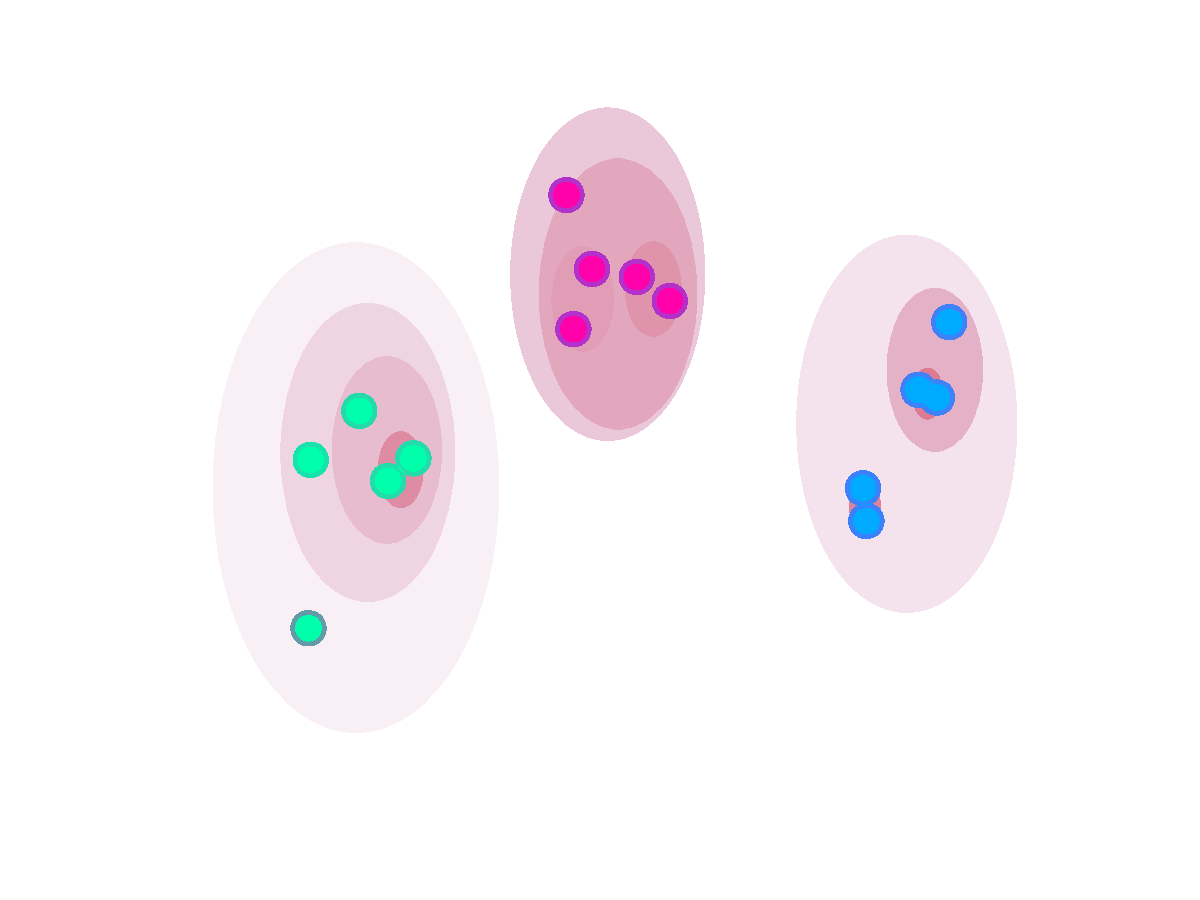
\includegraphics[width=\textwidth]{aglomerative}
\end{frame}


\begin{frame}{Кластеризация дивизимным анализом}{Divisive clustering}

\begin{itemize}
\item Более сложный по сравнению с агломеративной кластеризацией метод
\item Изначально все объекты содержатся в одном кластере
\item Кластер(ы) некоторым образом разбиваются дихотомически
\item С каждой итерацией количество кластеров увеличивается, процесс останавливается при достижении нужного их количества
\end{itemize}
\end{frame}



\begin{frame}{Дивизимная кластеризация}{}
\begin{block}{}
\small
{\bf\color{main}Вход:} множество объектов $\mathcal{X}$, параметр $k$ количества кластеров\\
{\bf\color{main}Выход:} множество пар (объект-кластер) \\
\begin{itemize}
	\item Все объекты из $\mathcal{X}$ отнести к одному классу из $\mathcal{C}$
	\item Пока количество кластеров меньше, чем $k$
	\begin{itemize}
%		\item Выбрать два наиболее близких по метрике кластера из $C$:
%		$$
%		(S_1,S_2) = \mathop{\arg \max}_{S_1,S_2 \in C, S_1 \ne S_2} \rho(S_1,S_2)
%		$$

		\item Разбить кластер с наибольшим внутрикластерным расстоянием на два с помощью какого-либо алгоритма кластеризации
	\end{itemize}
	\item Возвратить пары (объект из $\mathcal{X}$ -- номер кластера, в который попал этот объект)
\end{itemize}
\end{block}
\end{frame}

\section{}

\begin{frame}{Источники}
\begin{enumerate}
\item Воронцов, К.В. <<Лекции по алгоритмам кластеризации и многомерного шкалирования>>
\item Moore A. "K-means and Hierarchical Clustering"
\item Singh A. "Spectral Clustering"
\item Николенко С.И. <<Алгоритмы кластеризации>>
\item Ng A. "The k-means clustering algorithm"
\end{enumerate}
\end{frame}


\end{document}